%%%%%%%%%%%%%%%%%%%%%%%%%%%%%%%%%%%%%%%%%%%%%%%%%%%%%%%%%%%%%%%%%%%%%%%%%%%%%%%%
\begin{frame}[fragile]\frametitle{}
\begin{center}
{\Large Conclusion}
\end{center}
\end{frame}


%%%%%%%%%%%%%%%%%%%%%%%%%%%%%%%%%%%%%%%%%%%%%%%%%%%%%%%%%%%
\begin{frame}[fragile]\frametitle{Architecture}

\begin{columns}
    \begin{column}[T]{0.5\linewidth}
			\begin{center}
			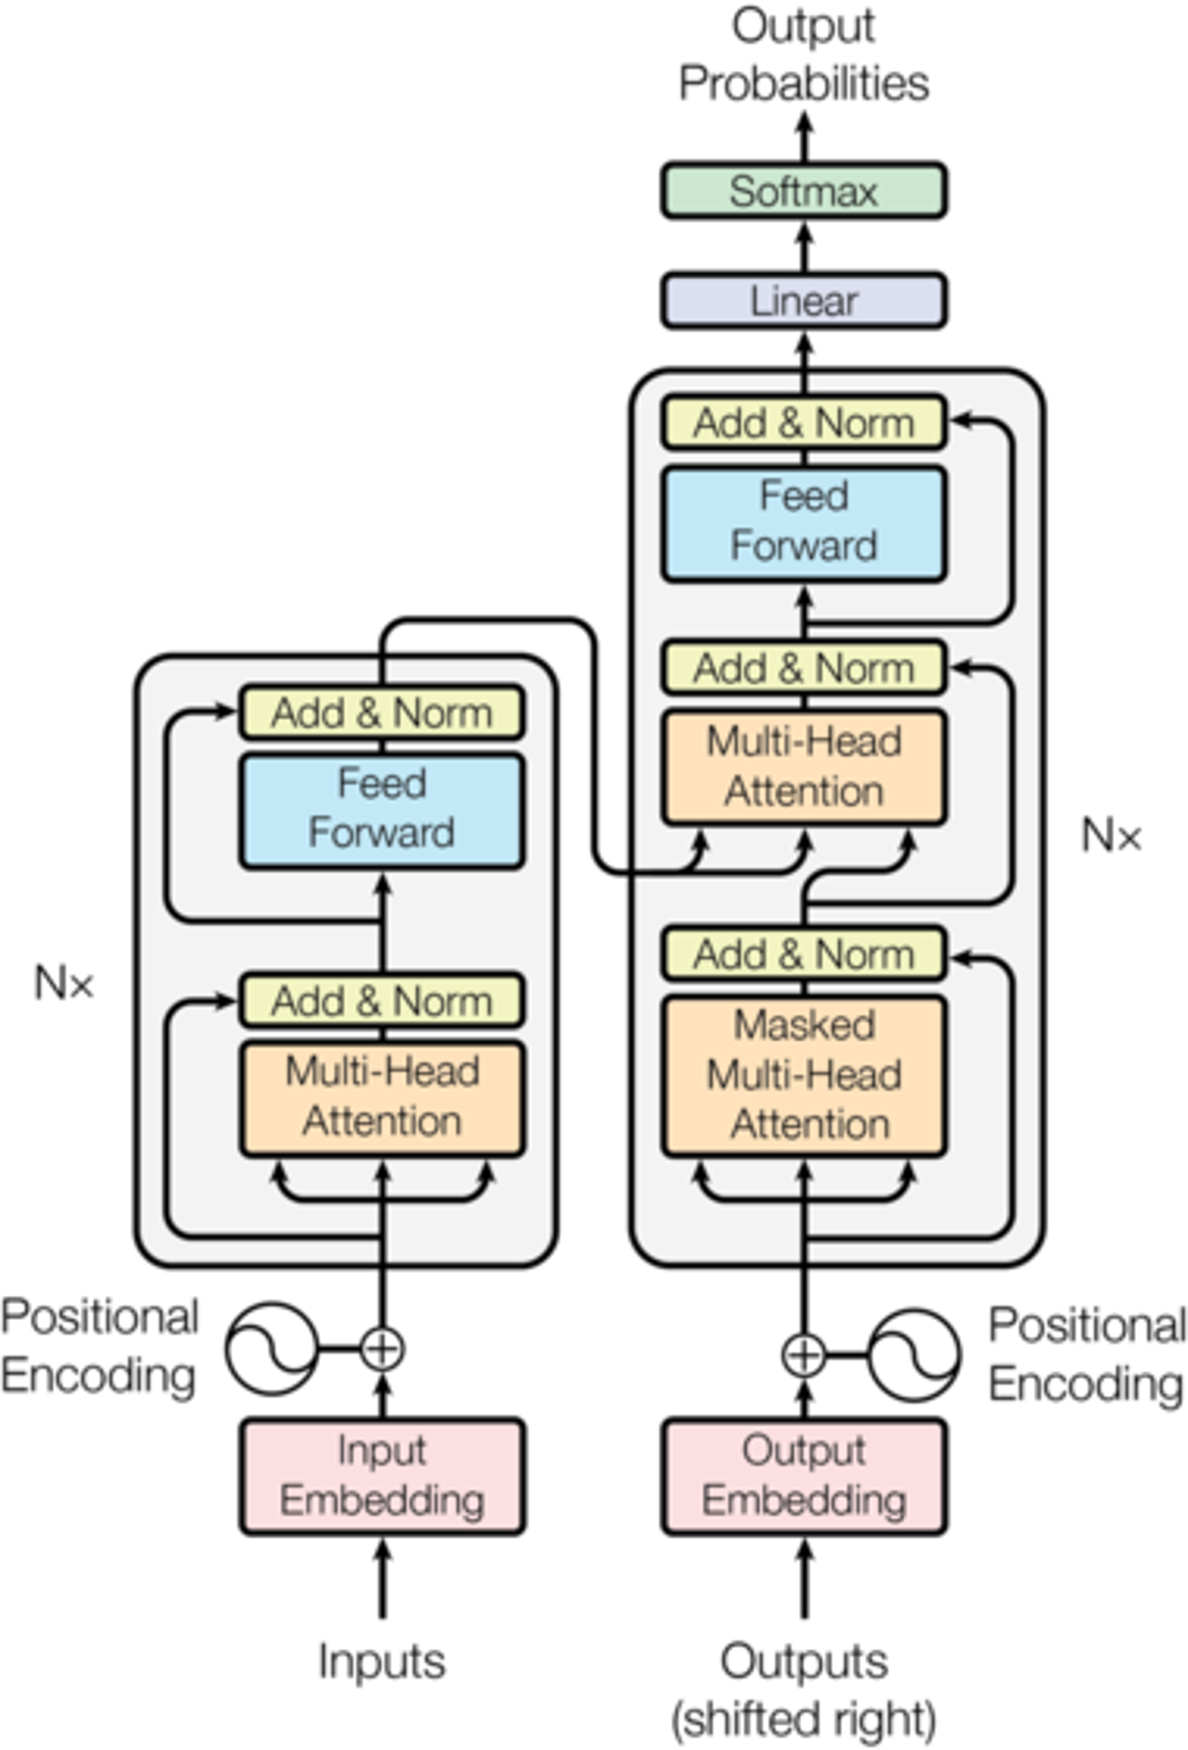
\includegraphics[width=0.8\linewidth,keepaspectratio]{bert65}
			\end{center}		
		\end{column}
    \begin{column}[T]{0.5\linewidth}
      \begin{itemize}
			\item Encoder-Decoder was there
			\item New?: Multi head attention
			\item Fine tuned with Custom Data
			\item Flavors:
      \begin{itemize}
			\item Encoder only: BERT, XLNet
			\item Decoder only
			\item Encoder-Decoder
			\end{itemize}
			\end{itemize}
    \end{column}
  \end{columns}
			
\end{frame}

%%%%%%%%%%%%%%%%%%%%%%%%%%%%%%%%%%%%%%%%%%%%%%%%%%%%%%%%%%%
\begin{frame}[fragile]\frametitle{Encoder only}

\begin{columns}
    \begin{column}[T]{0.5\linewidth}
			\begin{center}
			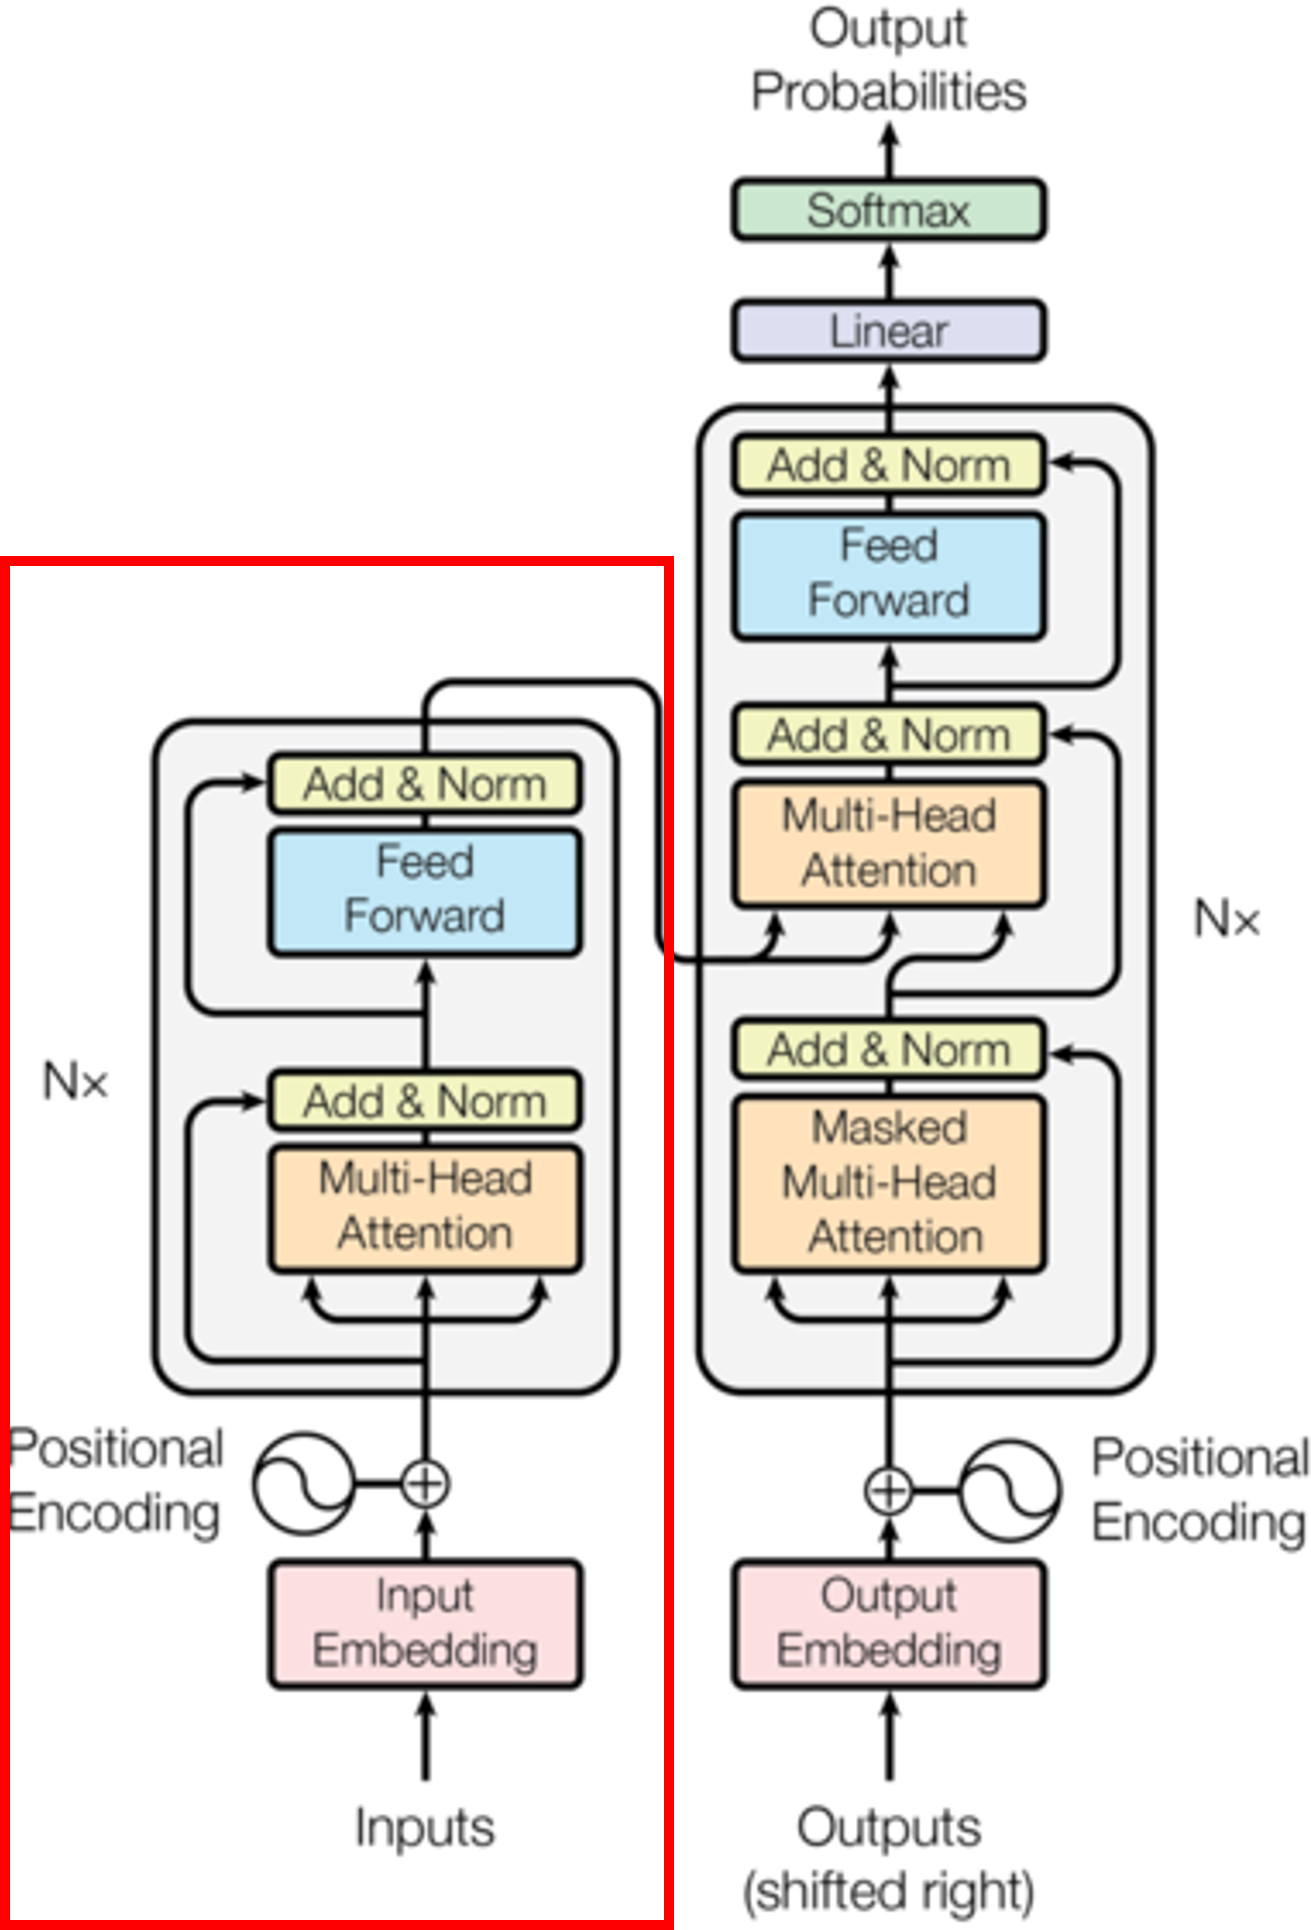
\includegraphics[width=0.8\linewidth,keepaspectratio]{bert66}
			\end{center}		
		\end{column}
    \begin{column}[T]{0.5\linewidth}
      \begin{itemize}
			\item If we are only interested in training a language model for the input for some other tasks, then we do not need the decoder of the transformer. 
			\item Pre-trained by predicting masked word
			\item BERT, XLNet, DistillBERT, RoBERTA
			\item Usage:
      \begin{itemize}
			\item Text Classification
			\item Named Entity Recognition
			\item Extractive Question Answering
			\end{itemize}
			\end{itemize}
    \end{column}
  \end{columns}
			
\end{frame}

%%%%%%%%%%%%%%%%%%%%%%%%%%%%%%%%%%%%%%%%%%%%%%%%%%%%%%%%%%%
\begin{frame}[fragile]\frametitle{Decoder only}

\begin{columns}
    \begin{column}[T]{0.5\linewidth}
			\begin{center}
			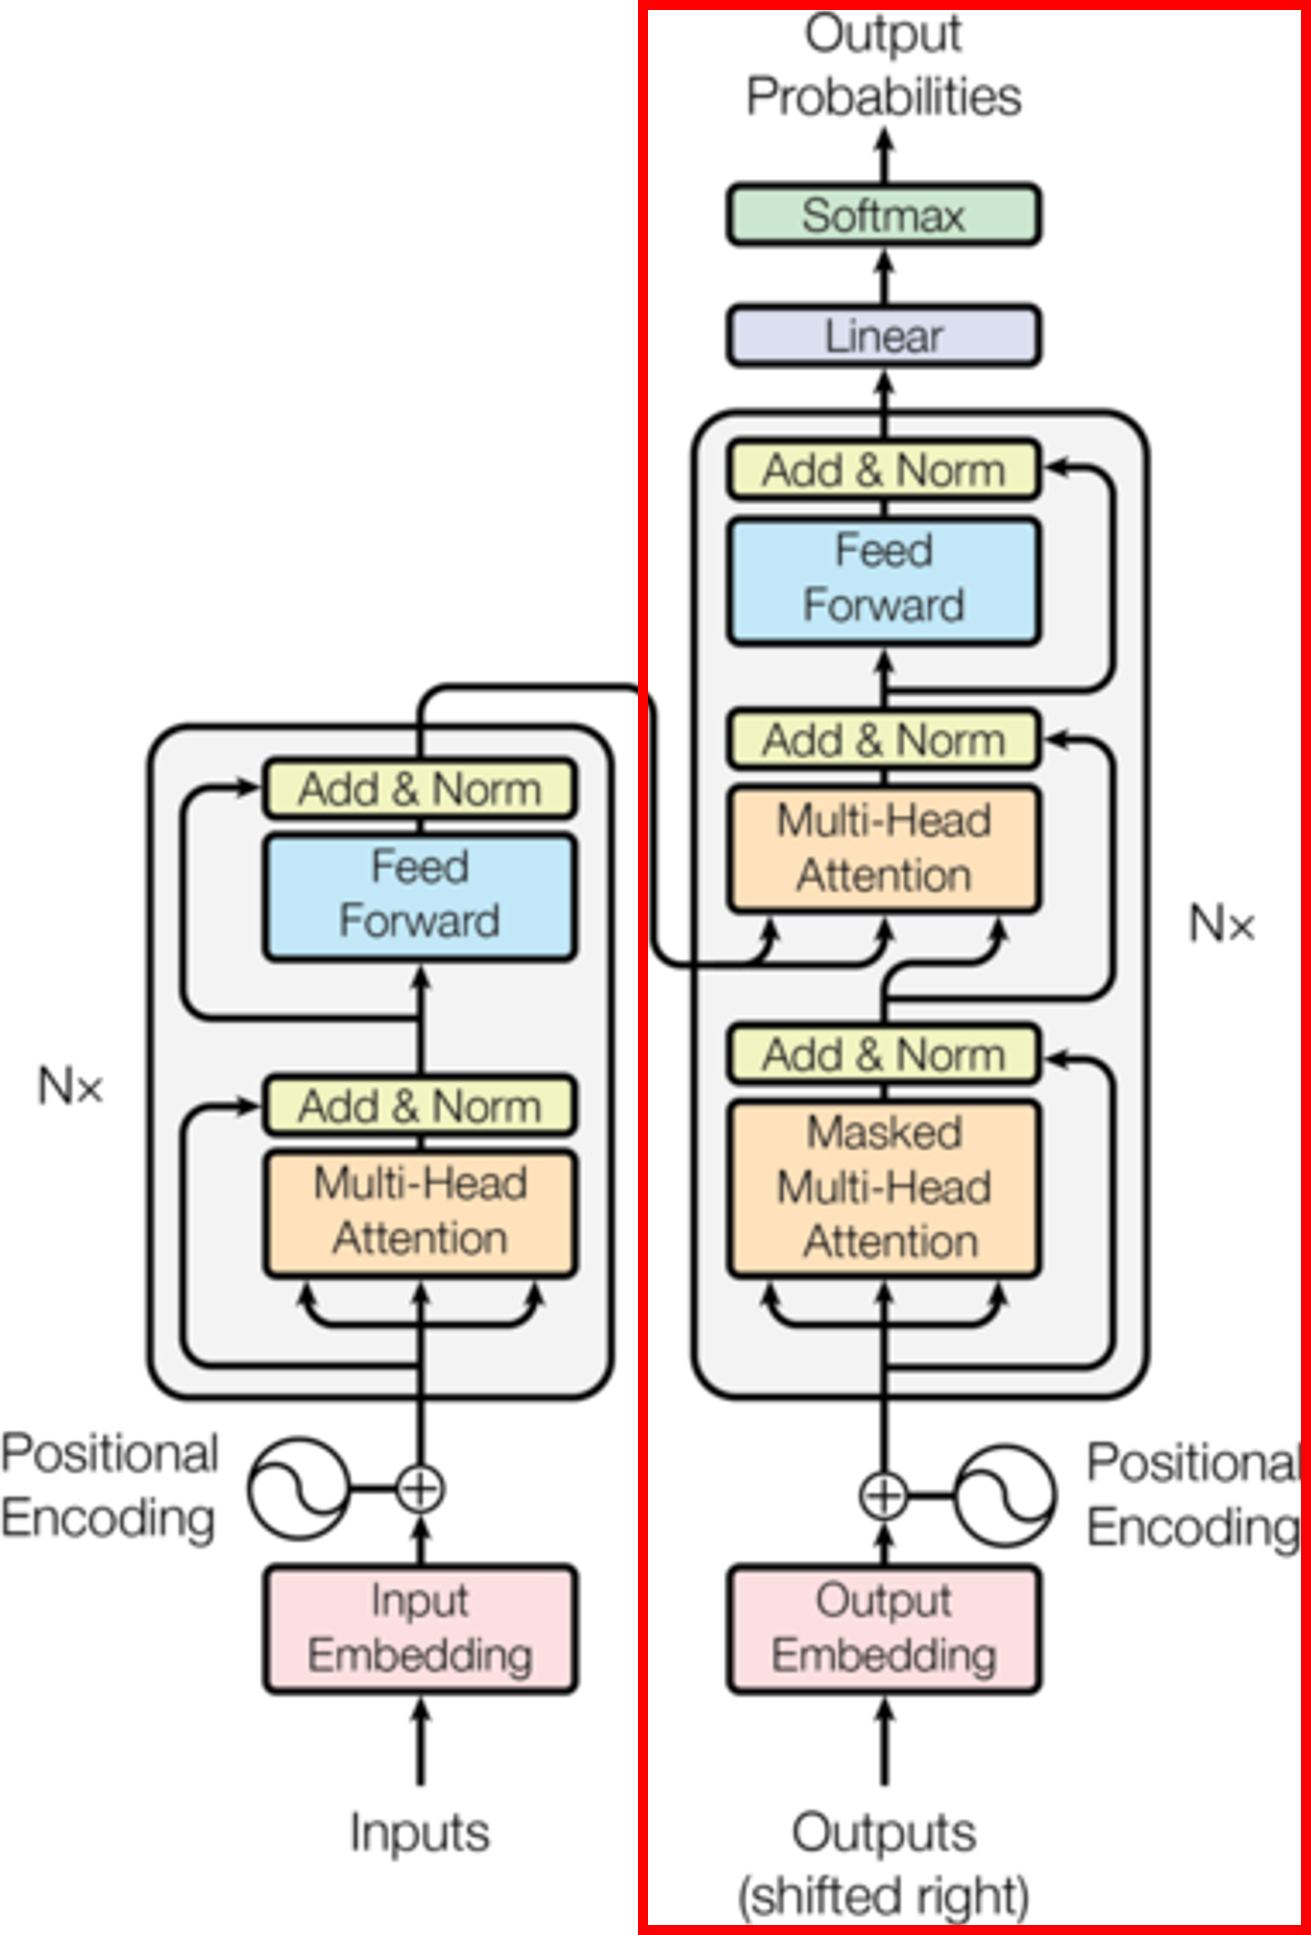
\includegraphics[width=0.8\linewidth,keepaspectratio]{bert67}
			\end{center}		
		\end{column}
    \begin{column}[T]{0.5\linewidth}
      \begin{itemize}
			\item If we do not have input, we just want to model the “next word”, we can get rid of the encoder side of a transformer and output “next word” one by one. 
			\item Pre-trained by predicting next word
			\item GPT-*, Transformer XL
			\item Usage:
      \begin{itemize}
			\item Text Generation
			\end{itemize}
			\end{itemize}
    \end{column}
  \end{columns}
			
\end{frame}

%%%%%%%%%%%%%%%%%%%%%%%%%%%%%%%%%%%%%%%%%%%%%%%%%%%%%%%%%%%
\begin{frame}[fragile]\frametitle{Encoder-Decoder, both}

\begin{columns}
    \begin{column}[T]{0.5\linewidth}
			\begin{center}
			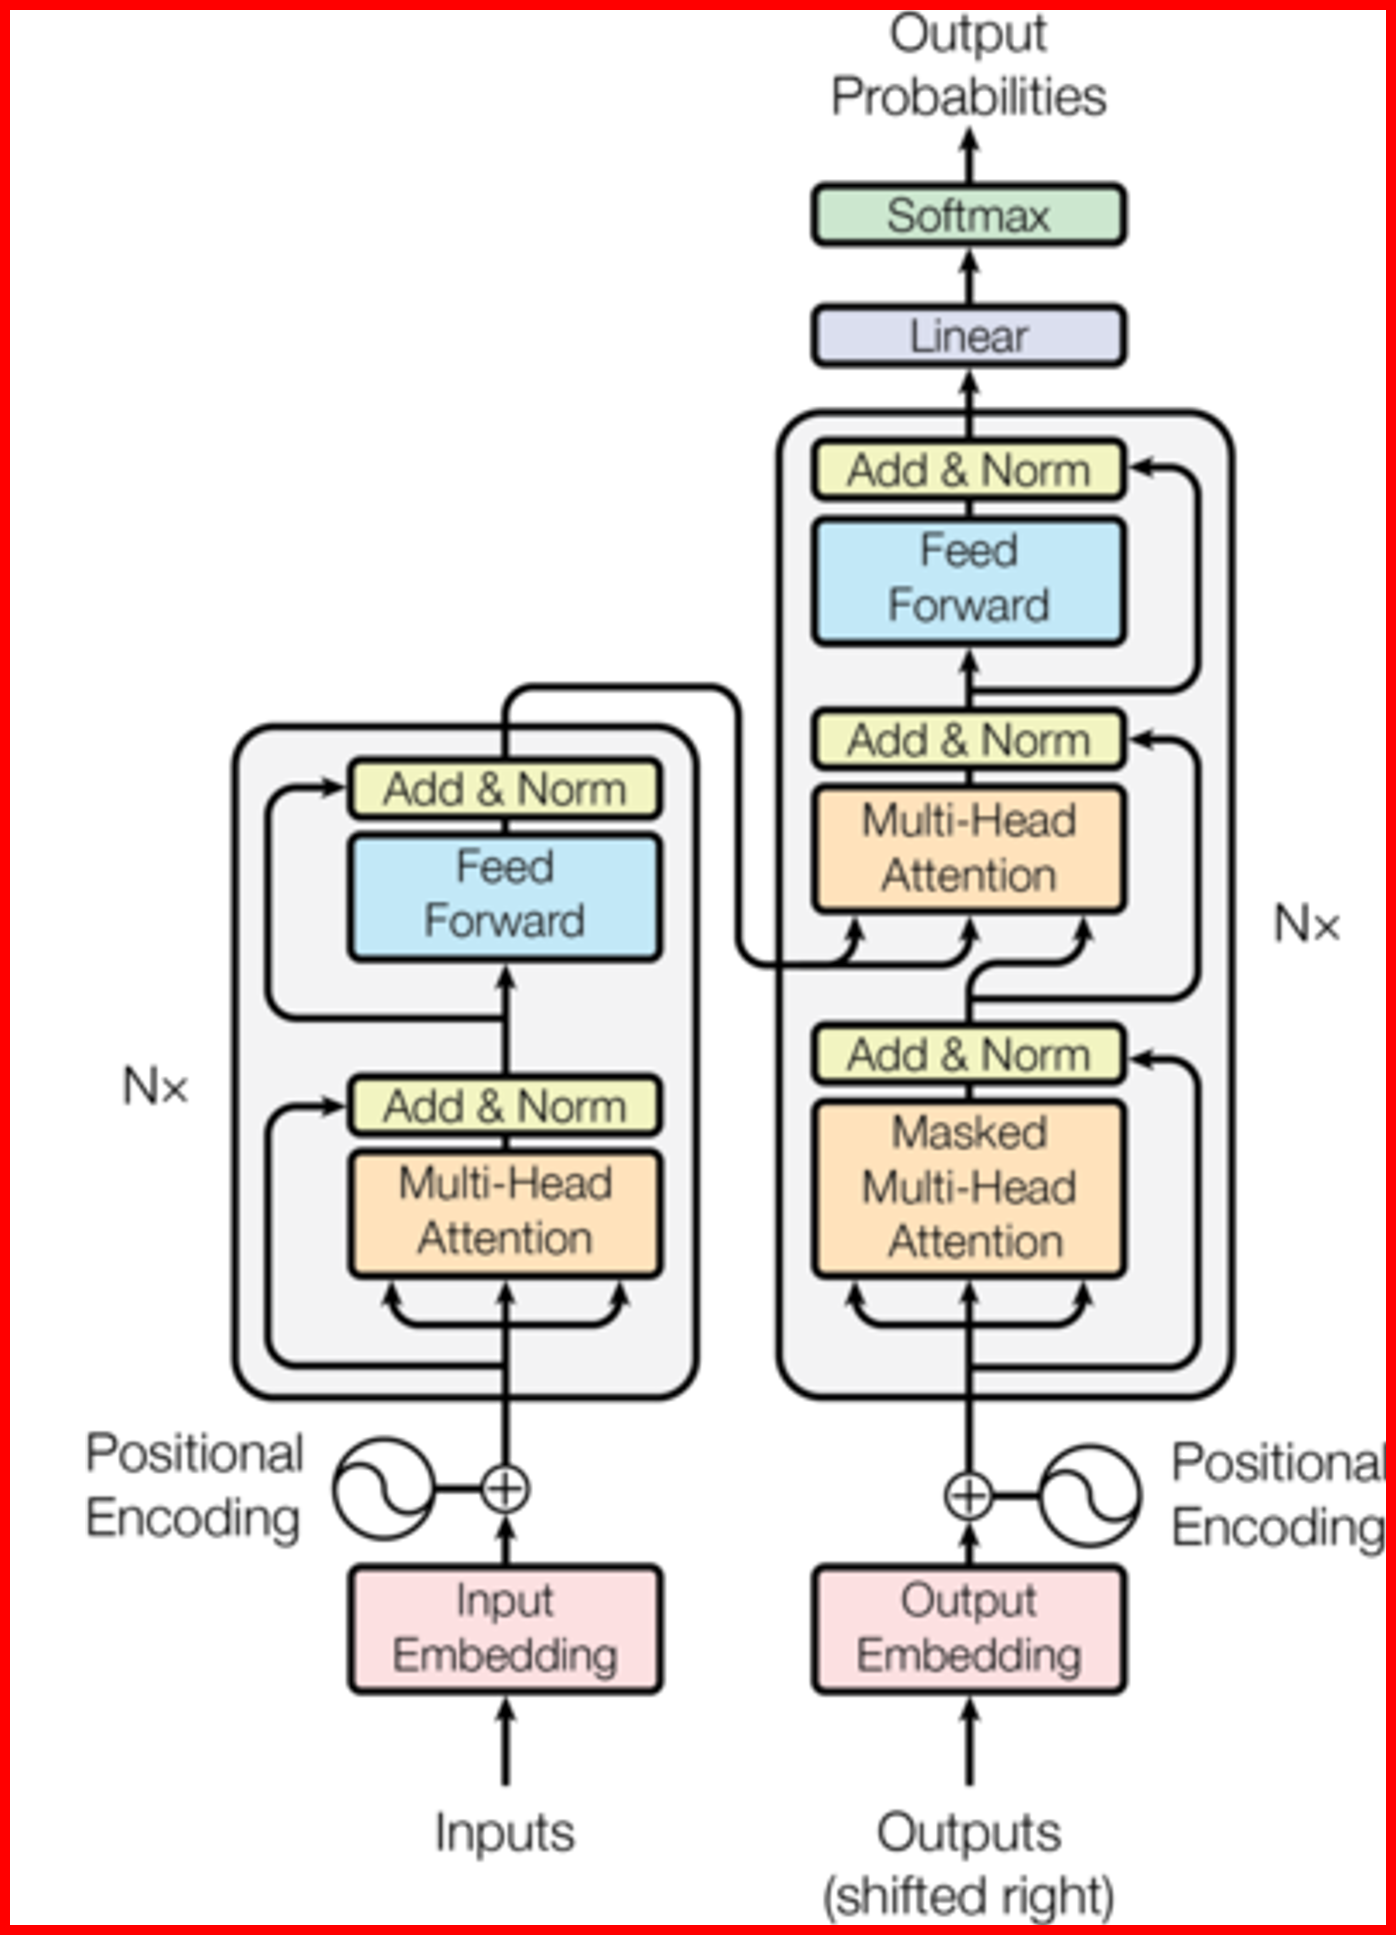
\includegraphics[width=0.8\linewidth,keepaspectratio]{bert68}
			\end{center}		
		\end{column}
    \begin{column}[T]{0.5\linewidth}
      \begin{itemize}
			\item Pre-trained by Seq2Seq manner
			\item T5, BART, PEGASUS
			\item Usage:
      \begin{itemize}
			\item Text summarization
			\item Machine Translation
			\item SQL generation
			\end{itemize}
			\end{itemize}
    \end{column}
  \end{columns}
			
\end{frame}






